\documentclass[11pt,a4paper]{article}

% --- Paquetes Esenciales ---
\usepackage[T1]{fontenc}
\usepackage[utf8]{inputenc}
\usepackage[spanish,es-tabla]{babel}
\usepackage[margin=2.5cm]{geometry}
\usepackage{graphicx}
\usepackage{xcolor}
\usepackage{tcolorbox}
\tcbuselibrary{skins}
\usepackage{hyperref}
\usepackage{fancyhdr}
\usepackage{float}
\usepackage{booktabs}
\usepackage{titlesec}
\usepackage{enumitem}
\usepackage{tabularx}
\usepackage{caption}
\usepackage{subcaption}
\usepackage{amsmath}

% --- Colores Institucionales y Estilo Visual ---
\definecolor{unsaacblue}{RGB}{18, 52, 102}
\definecolor{cgbnavy}{RGB}{11, 37, 69}
\definecolor{cgbteal}{RGB}{19, 154, 140}
\definecolor{boxbg}{RGB}{248, 250, 252}
\definecolor{boxborder}{RGB}{203, 213, 225}

\hypersetup{
    colorlinks=true,
    linkcolor=unsaacblue,
    filecolor=unsaacblue,
    urlcolor=unsaacblue,
    citecolor=unsaacblue
}

% --- Encabezados y Pies de Página ---
\pagestyle{fancy}
\fancyhf{}
\fancyhead[L]{\small\textbf{UNSAAC} -- Ingeniería de Software I}
\fancyhead[R]{\small\textbf{Laboratorio 6}: Gestión de Flujo con Kanban (CGB Academy)}
\fancyfoot[L]{\small\textbf{Grupo de Laboratorio} -- Semestre 2026-I}
\fancyfoot[R]{\thepage}
\renewcommand{\headrulewidth}{0.8pt}
\renewcommand{\footrulewidth}{0.4pt}

% --- Formato de Títulos ---
\titleformat{\section}{\Large\bfseries\color{unsaacblue}}{\thesection.}{0.5em}{}[\titlerule]
\titleformat{\subsection}{\large\bfseries\color{unsaacblue}}{\thesubsection.}{0.5em}{}
\titleformat{\subsubsection}{\normalsize\bfseries\color{unsaacblue}}{\thesubsubsection.}{0.5em}{}

% --- Cajas de Texto Destacadas ---
\newtcolorbox{infobox}[1]{
    colback=boxbg,
    colframe=unsaacblue,
    fonttitle=\bfseries\color{white},
    title={#1},
    arc=2mm,
    boxrule=1pt,
    left=10pt, right=10pt, top=8pt, bottom=8pt,
    enhanced
}

\begin{document}

% ==============================================================================
% CARÁTULA INSTITUCIONAL
% ==============================================================================
\begin{titlepage}
    \centering
    {\Large\textbf{UNIVERSIDAD NACIONAL DE SAN ANTONIO ABAD DEL CUSCO}}\\[0.25cm]
    {\large\textbf{FACULTAD DE INGENIERÍA ELÉCTRICA, ELECTRÓNICA, INFORMÁTICA Y MECÁNICA}}\\[0.15cm]
    {\large\textbf{ESCUELA PROFESIONAL DE INGENIERÍA INFORMÁTICA Y DE SISTEMAS}}\\[0.8cm]

    
\includegraphics[width=4.2cm]{capturas/logo_unsaac.png}\\[0.8cm]

    {\Large\textbf{INFORME DE LABORATORIO N° 6}}\\[0.3cm]
    {\LARGE\textbf{\color{unsaacblue}Gestión del Flujo de Trabajo con Tablero Kanban}}\\[0.2cm]
    {\large\textbf{Proyecto: Centro de Capacitación e Inducción -- CGB Academy}}\\[0.15cm]
    {\normalsize Control de Flujo Continuo, Límites WIP, Cuellos de Botella y Métricas Ágiles}\\[0.8cm]

    \begin{infobox}{Datos de la Asignatura}
        \textbf{Curso:} Ingeniería de Software I (IF614)\\
        \textbf{Docente:} Ing. Lisha Sabah Diaz Caceres\\
        \textbf{Semestre Académico:} 2026-I\\
        \textbf{Repositorio Oficial:} \url{https://github.com/milith0kun/proyecto-ing-software}
    \end{infobox}

    \vspace{0.4cm}

    \textbf{\large Integrantes del Grupo:}\\[0.2cm]
    \begin{tabularx}{\textwidth}{c X c c}
        \toprule
        \textbf{N°} & \textbf{Apellidos y Nombres} & \textbf{Código} & \textbf{Correo Institucional} \\
        \midrule
        1 & Barazorda Cuellar, Hector & 145003 & 145003@unsaac.edu.pe \\
        2 & Carpio Hermoza, Alex & 164563 & 164563@unsaac.edu.pe \\
        3 & Quispe Mamani, Domingo de Guzman & 191978 & 191978@unsaac.edu.pe \\
        4 & Saire Bustamante, Edmil Jampier & 174449 & 174449@unsaac.edu.pe \\
        5 & Ticona Jancco, Ronaldo & 211816 & 211816@unsaac.edu.pe \\
        \bottomrule
    \end{tabularx}

    \vfill
    {\small Cusco, Perú -- 2026}
\end{titlepage}

\tableofcontents
\newpage

% ==============================================================================
% 1. OBJETIVO DEL LABORATORIO
% ==============================================================================
\section{Objetivo del Laboratorio}

El objetivo central del presente laboratorio es diseñar, implementar y gestionar de forma práctica el flujo de trabajo continuo del equipo de desarrollo para la plataforma web \textbf{CGB Academy} (Centro de Capacitación e Inducción de CIIP Latam, GEOMINA Latam y BIOMEDIC) mediante un \textbf{Tablero Kanban}.

Específicamente, se busca:
\begin{enumerate}[label=\alph*)]
    \item Estructurar formalmente las columnas y transiciones de estado del ciclo de desarrollo de software desde el Backlog hasta el Despliegue en Producción.
    \item Asignar las historias de usuario prioritarias del proyecto a miembros específicos del equipo de desarrollo según los roles acordados para el Sprint 1.
    \item Implementar restricciones de trabajo en curso (\textit{Work In Progress} -- WIP) por columna para prevenir la sobrecarga cognitiva y optimizar el rendimiento del equipo.
    \item Identificar cuellos de botella mediante la simulación de flujo continuo en fases de revisión de código (\textit{Code Review}).
    \item Cuantificar y analizar las métricas fundamentales de Kanban: \textit{Lead Time}, \textit{Cycle Time}, \textit{Throughput} y Diagrama de Flujo Acumulado (\textit{Cumulative Flow Diagram} -- CFD).
\end{enumerate}

% ==============================================================================
% 2. FUNDAMENTO TEÓRICO
% ==============================================================================
\section{Fundamento Teórico}

\subsection{El Método Kanban en la Ingeniería de Software}
Kanban es un método evolutivo y no disruptivo para gestionar y mejorar el trabajo en servicios de entrega de valor intelectual. A diferencia de marcos iterativos con ciclos de tiempo fijos (*time-boxes* como Scrum puro), Kanban se fundamenta en los siguientes principios:
\begin{itemize}
    \item \textbf{Visualizar el trabajo:} Modelar de forma gráfica el flujo mediante columnas que representen estados reales del ciclo de vida del software.
    \item \textbf{Limitar el trabajo en progreso (WIP):} Evitar el desperdicio generado por el cambio de contexto (*multitasking* ineficiente) y garantizar que las tareas se completen antes de iniciar nuevas (*Stop Starting, Start Finishing*).
    \item \textbf{Gestionar el flujo:} Medir el movimiento de las historias a través de las etapas para eliminar fricciones y demoras.
    \item \textbf{Hacer explícitas las políticas de proceso:} Establecer definiciones claras de ``Listo para pasar'' (*Definition of Done* y criterios de transición entre columnas).
    \item \textbf{Implementar ciclos de retroalimentación:} Monitorear indicadores cuantitativos para la toma de decisiones basada en datos empíricos.
\end{itemize}

\subsection{Flujo Continuo y Ley de Little}
El flujo continuo persigue que una unidad de trabajo transite desde su solicitud hasta su entrega sin interrupciones ni tiempos muertos. En la teoría de colas y gestión de operaciones, este comportamiento está gobernado por la \textbf{Ley de Little}:
\begin{equation}
    \text{WIP} = \text{Throughput} \times \text{Cycle Time}
\end{equation}
Donde:
\begin{itemize}
    \item $\text{WIP}$ es el número promedio de elementos que se encuentran activos en el sistema.
    \item $\text{Throughput}$ ($\lambda$) es la tasa de entrega o rendimiento del equipo (historias terminadas por unidad de tiempo).
    \item $\text{Cycle Time}$ ($W$) es el tiempo promedio que una tarea permanece dentro del sistema productivo.
\end{itemize}
De esta relación matemática se desprende una conclusión crítica: al reducir el límite de WIP manteniendo constante el Throughput, el tiempo de ciclo disminuye proporcionalmente, acelerando la entrega de valor al usuario final.

\subsection{Métricas Clave: Lead Time y Cycle Time}
Para evaluar la eficiencia del proceso se distinguen dos medidas temporales cardinales:
\begin{itemize}
    \item \textbf{Lead Time (Tiempo de Entrega):} Lapso total transcurrido desde que el usuario o Product Owner concibe e ingresa la necesidad al Backlog hasta que la funcionalidad está disponible en producción para los colaboradores de CGB Academy.
    \item \textbf{Cycle Time (Tiempo de Ciclo):} Subintervalo que abarca únicamente desde que un desarrollador toma la tarjeta e inicia la codificación activa (*En Progreso*) hasta que la historia supera las pruebas y la revisión de código (*Terminado*).
\end{itemize}

\begin{figure}[H]
    \centering
    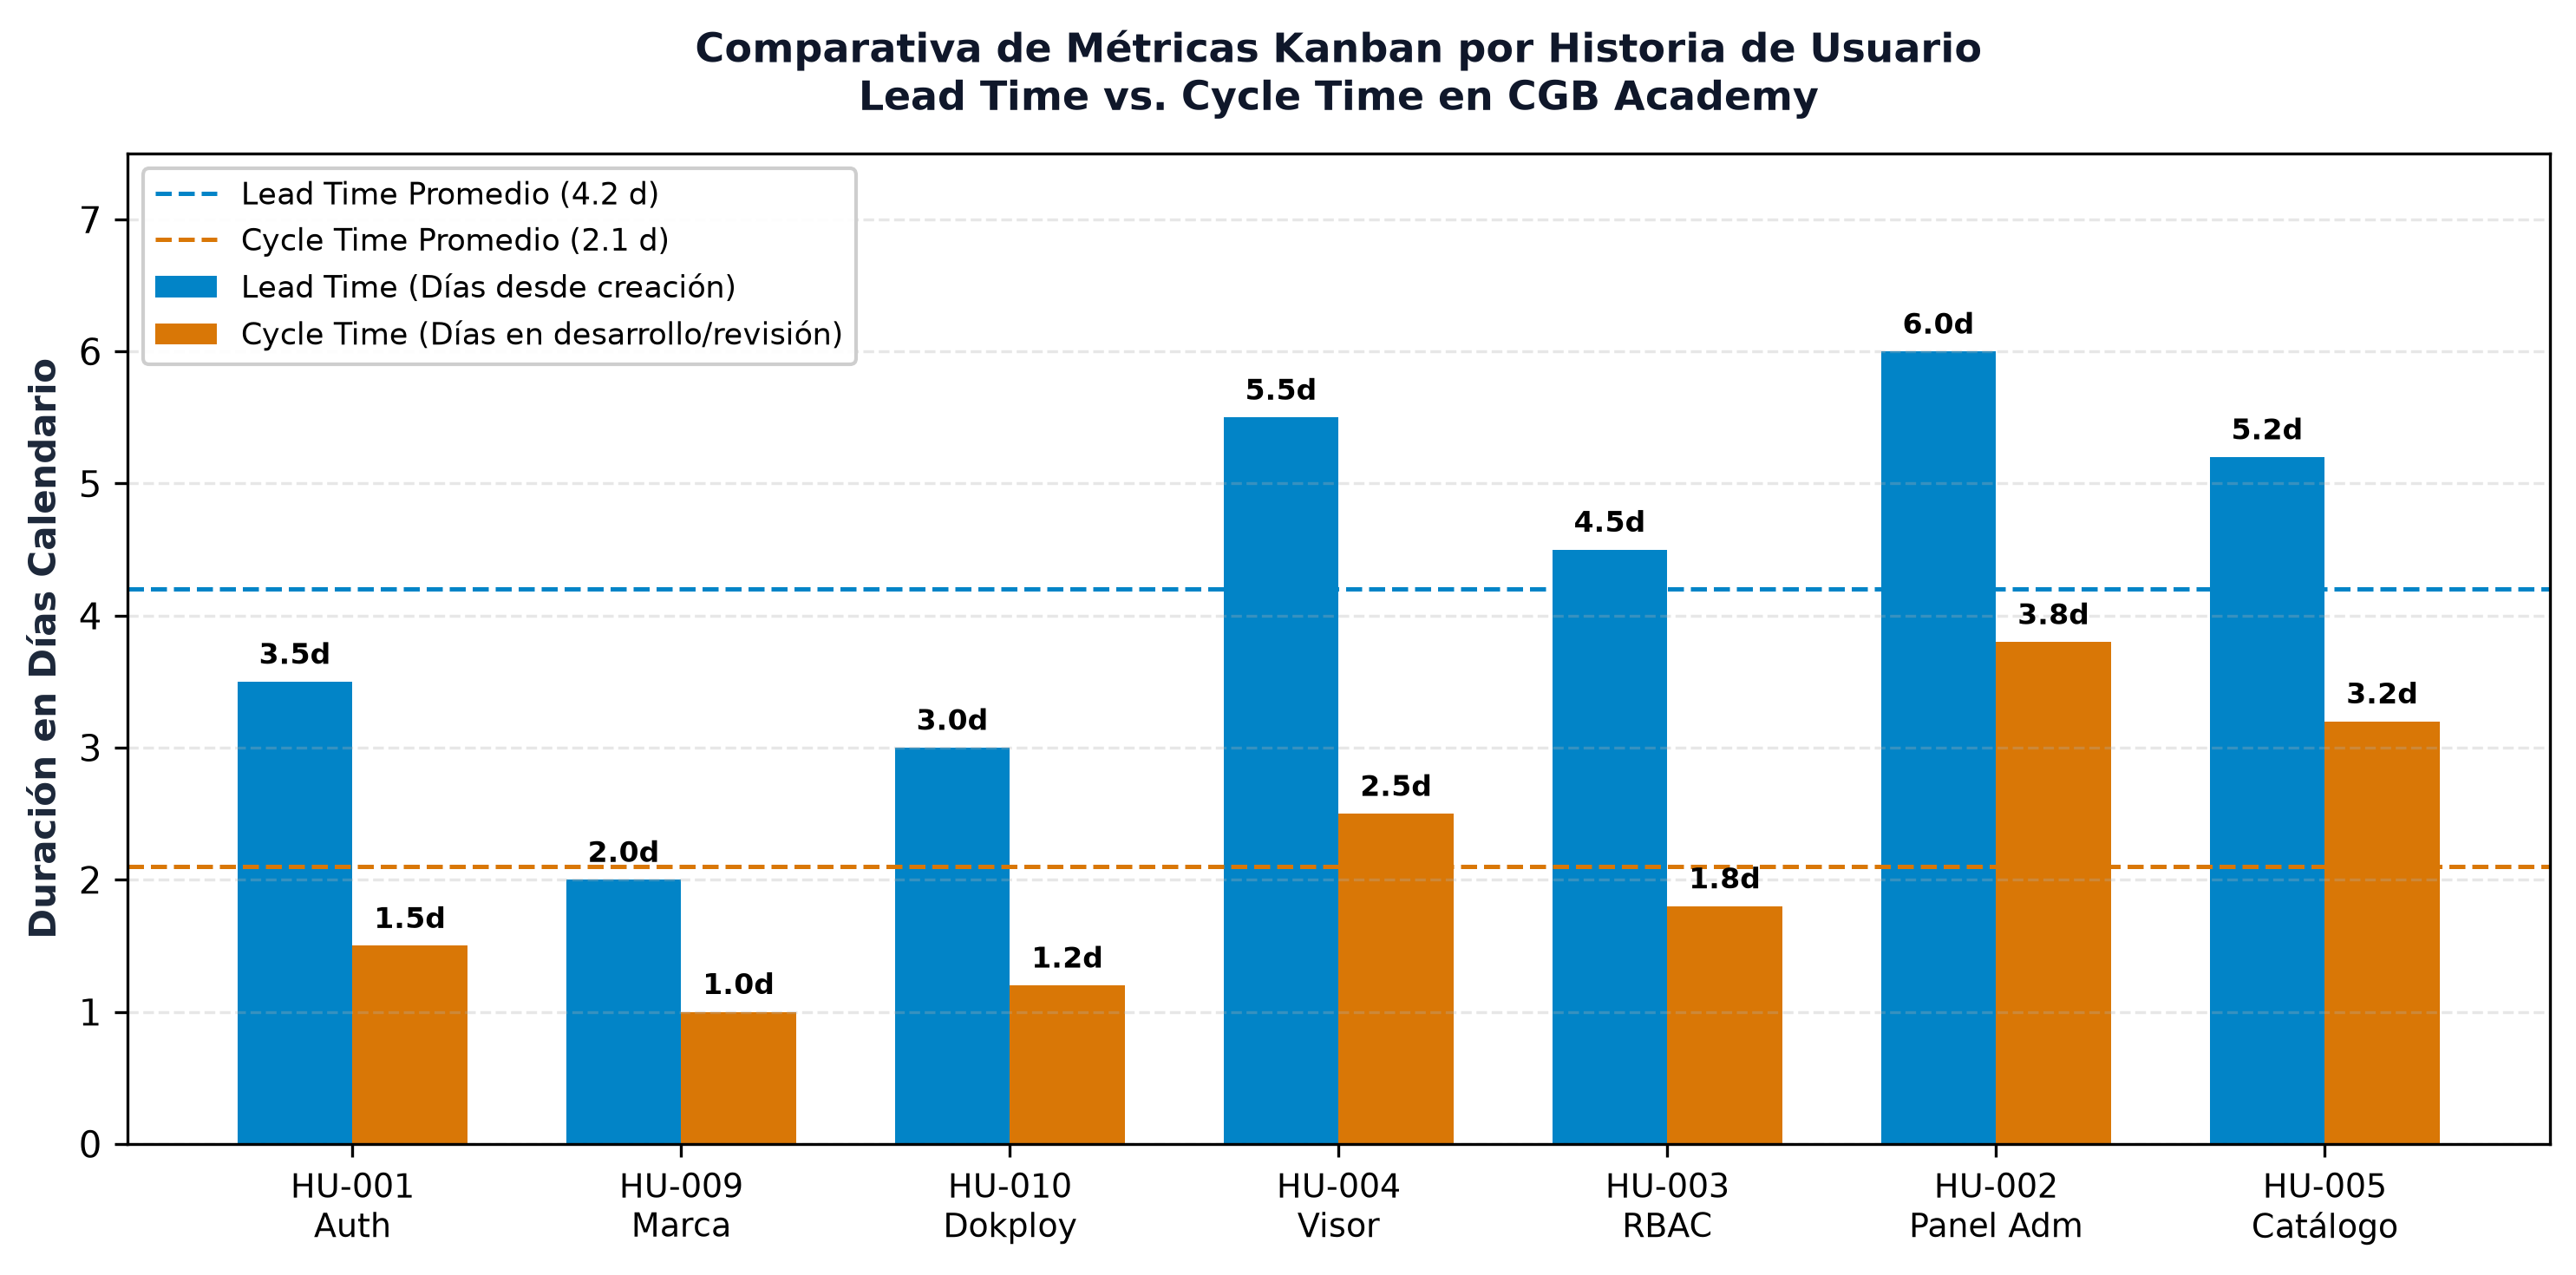
\includegraphics[width=0.88\textwidth]{capturas/metricas_lead_cycle_cgb.png}
    \caption{Comparativa de Métricas: Lead Time vs. Cycle Time por Historia de Usuario en el Proyecto CGB Academy.}
    \label{fig:metricas_lead_cycle}
\end{figure}

% ==============================================================================
% 3. HERRAMIENTAS UTILIZADAS
% ==============================================================================
\section{Herramientas Utilizadas}
\begin{itemize}
    \item \textbf{Jira Software / GitHub Projects Kanban:} Plataforma para la creación de tableros ágiles, parametrización de columnas, configuración de límites WIP, asignación de responsables y seguimiento de incidencias.
    \item \textbf{Git \& GitHub CLI (\texttt{gh}):} Control de versiones distribuido con ramas dedicadas por colaborador (\texttt{edmil-saire}, \texttt{hector-barazorda}, etc.) para validar el flujo de Pull Requests.
    \item \textbf{Python 3 \& Matplotlib / Seaborn:} Generación automatizada de tableros, diagramas de flujo acumulado (CFD) y gráficos analíticos de dispersión de tiempos.
    \item \textbf{Next.js 15, Prisma ORM y MongoDB Atlas:} Código base del proyecto CGB Academy sobre el cual se ejecutan y validan las historias de usuario descritas en el tablero.
\end{itemize}

\newpage

% ==============================================================================
% 4. ACTIVIDADES DESARROLLADAS
% ==============================================================================
\section{Actividades Desarrolladas}

\subsection{Parte 1: Diseño del Tablero Kanban}
Para reflejar fielmente la dinámica técnica de desarrollo de software en CGB Academy, se diseñaron cinco columnas secuenciales con políticas de transición explícitas, tal como se resume en el Cuadro~\ref{tab:columnas_politicas}.

\begin{table}[H]
    \centering
    \small
    \caption{Estructura de Columnas, Límites WIP y Políticas de Transición del Tablero.}
    \label{tab:columnas_politicas}
    \begin{tabularx}{\textwidth}{p{3.2cm} c p{4.2cm} X}
        \toprule
        \textbf{Columna (Estado)} & \textbf{Límite WIP} & \textbf{Definición de Entrada} & \textbf{Criterio de Salida (Pull)} \\
        \midrule
        \textbf{1. Backlog} & Sin límite ($\infty$) & Historias documentadas en Agile Inception con estimación en Story Points. & Historia refinada y priorizada por el Product Owner para el sprint en curso. \\
        \addlinespace
        \textbf{2. Por Hacer (To Do)} & Máx. 3 & Historias seleccionadas listas para ser abordadas por los ingenieros. & Desarrollador con capacidad disponible toma la tarjeta e inicia la rama Git. \\
        \addlinespace
        \textbf{3. En Progreso} & Máx. 2 & Código en implementación activa en entorno de desarrollo local. & Suite de pruebas unitarias exitosas y Pull Request (PR) abierto en GitHub. \\
        \addlinespace
        \textbf{4. En Revisión (PR)} & Máx. 2 & PR creado solicitando revisión de pares (*Peer Code Review*). & Aprobación de al menos un revisor técnico y pruebas de integración superadas. \\
        \addlinespace
        \textbf{5. Terminado (Done)} & Sin límite ($\infty$) & Merge realizado en la rama \texttt{main} y verificado en entorno de staging. & Despliegue operativo en servidor VPS Dokploy y aceptación funcional. \\
        \bottomrule
    \end{tabularx}
\end{table}

\subsection{Parte 2: Configuración del Flujo y Asignación de Responsables}
Se tomaron las Historias de Usuario (HU) del proyecto de capacitación institucional, vinculándolas a cada miembro del equipo de acuerdo a los roles de trabajo del Sprint 1:

\begin{itemize}
    \item \textbf{HU-001 (Autenticación Segura y RBAC):} Asignada a \textit{Saire Bustamante, Edmil} (Product Owner / Dev Full-Stack). Estado: \textbf{Terminado}.
    \item \textbf{HU-002 (Panel Administrativo de Creación de Capacitaciones):} Asignada a \textit{Quispe Mamani, Domingo}. Estado: \textbf{En Revisión} (Bloqueada por límite WIP).
    \item \textbf{HU-003 (Gestión de Usuarios y Roles en MongoDB):} Asignada a \textit{Barazorda Cuellar, Hector} (Scrum Master / Dev Full-Stack). Estado: \textbf{En Progreso}.
    \item \textbf{HU-004 (Visor de Diapositivas Interactivas y Cronómetro):} Asignada a \textit{Saire Bustamante, Edmil}. Estado: \textbf{En Progreso}.
    \item \textbf{HU-005 (Catálogo Público Multi-marca: CIIP, GEOMINA, BIOMEDIC):} Asignada a \textit{Carpio Hermoza, Alex}. Estado: \textbf{En Revisión} (Saturando columna).
    \item \textbf{HU-006 (Generación de Certificados Digitales con QR):} Asignada a \textit{Ticona Jancco, Ronaldo}. Estado: \textbf{Backlog}.
    \item \textbf{HU-009 (Sistema de Diseño y Tokens CSS Institucionales):} Asignada a \textit{Ticona Jancco, Ronaldo}. Estado: \textbf{Terminado}.
    \item \textbf{HU-010 (Automatización de Despliegue en Dokploy):} Asignada a \textit{Saire Bustamante, Edmil}. Estado: \textbf{Terminado}.
\end{itemize}

\begin{figure}[H]
    \centering
    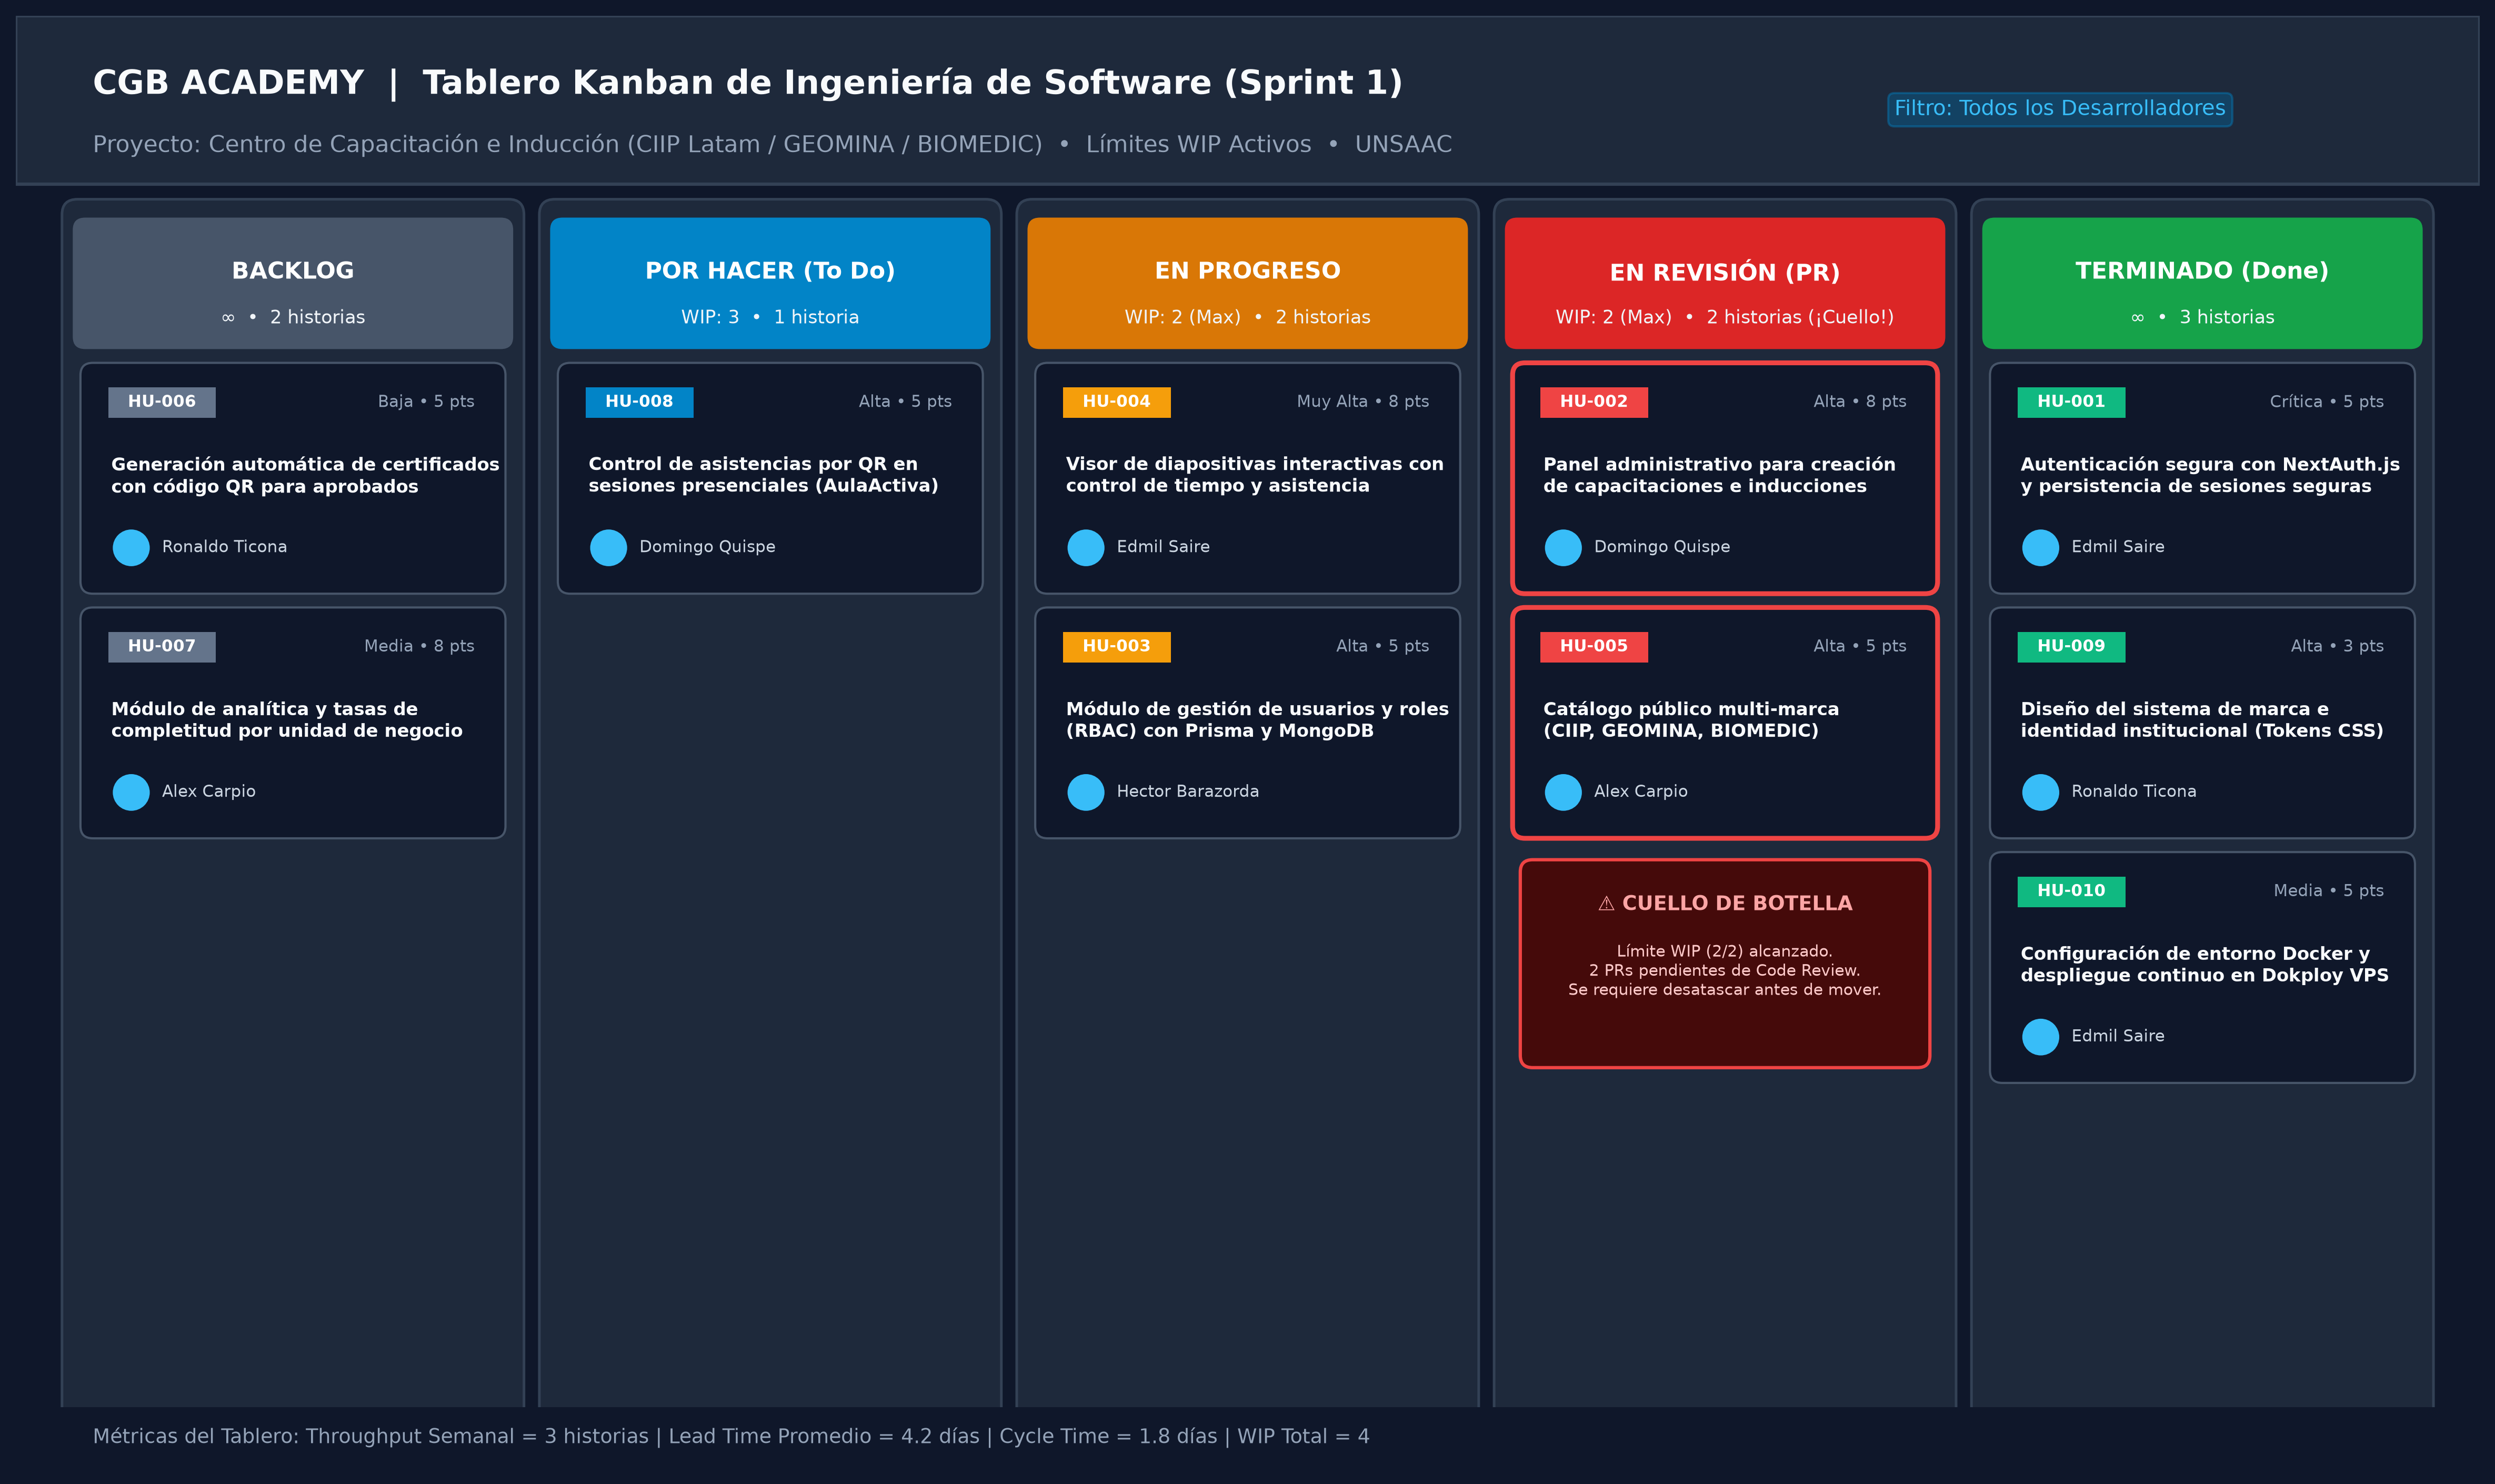
\includegraphics[width=\textwidth]{capturas/tablero_kanban_cgb.png}
    \caption{Visualización Integral del Tablero Kanban de CGB Academy con Límites WIP y Alerta de Cuello de Botella.}
    \label{fig:tablero_kanban}
\end{figure}

\subsection{Parte 3: Simulación de Flujo y Detección de Cuellos de Botella}
Durante la simulación de ejecución del sprint se identificó un evento crítico:
\begin{infobox}{Análisis del Cuello de Botella Detectado}
    \textbf{Ubicación:} Columna \textit{En Revisión (Code Review)}.\\
    \textbf{Síntoma:} Las historias HU-002 y HU-005 alcanzaron el límite estricto de $\text{WIP} = 2$. Dos desarrolladores culminaron su codificación e intentaron mover nuevas tareas a revisión, violando el límite configurado.\\
    \textbf{Causa Raíz:} Los revisores asignados (Scrum Master y Product Owner) se encontraban concentrados en tareas pesadas de desarrollo (\textit{En Progreso}), generando un tapón en la integración de Pull Requests.\\
    \textbf{Acción Correctiva Kanban (*Swarming*):} El equipo detuvo la incorporación de nuevas historias desde ``Por Hacer'' y aplicó la política de enjambre: el Product Owner pausó el desarrollo de HU-004 durante 4 horas para revisar y aprobar el PR de HU-005, liberando la capacidad de la columna de revisión.
\end{infobox}

% ==============================================================================
% 5. DIAGRAMA DE FLUJO ACUMULADO (CFD) Y ANÁLISIS
% ==============================================================================
\section{Diagrama de Flujo Acumulado (CFD) y Análisis de Rendimiento}

El Diagrama de Flujo Acumulado (\textit{Cumulative Flow Diagram} -- CFD) constituye la herramienta analítica más potente de Kanban para evaluar la estabilidad del sistema productivo a lo largo del tiempo.

\begin{figure}[H]
    \centering
    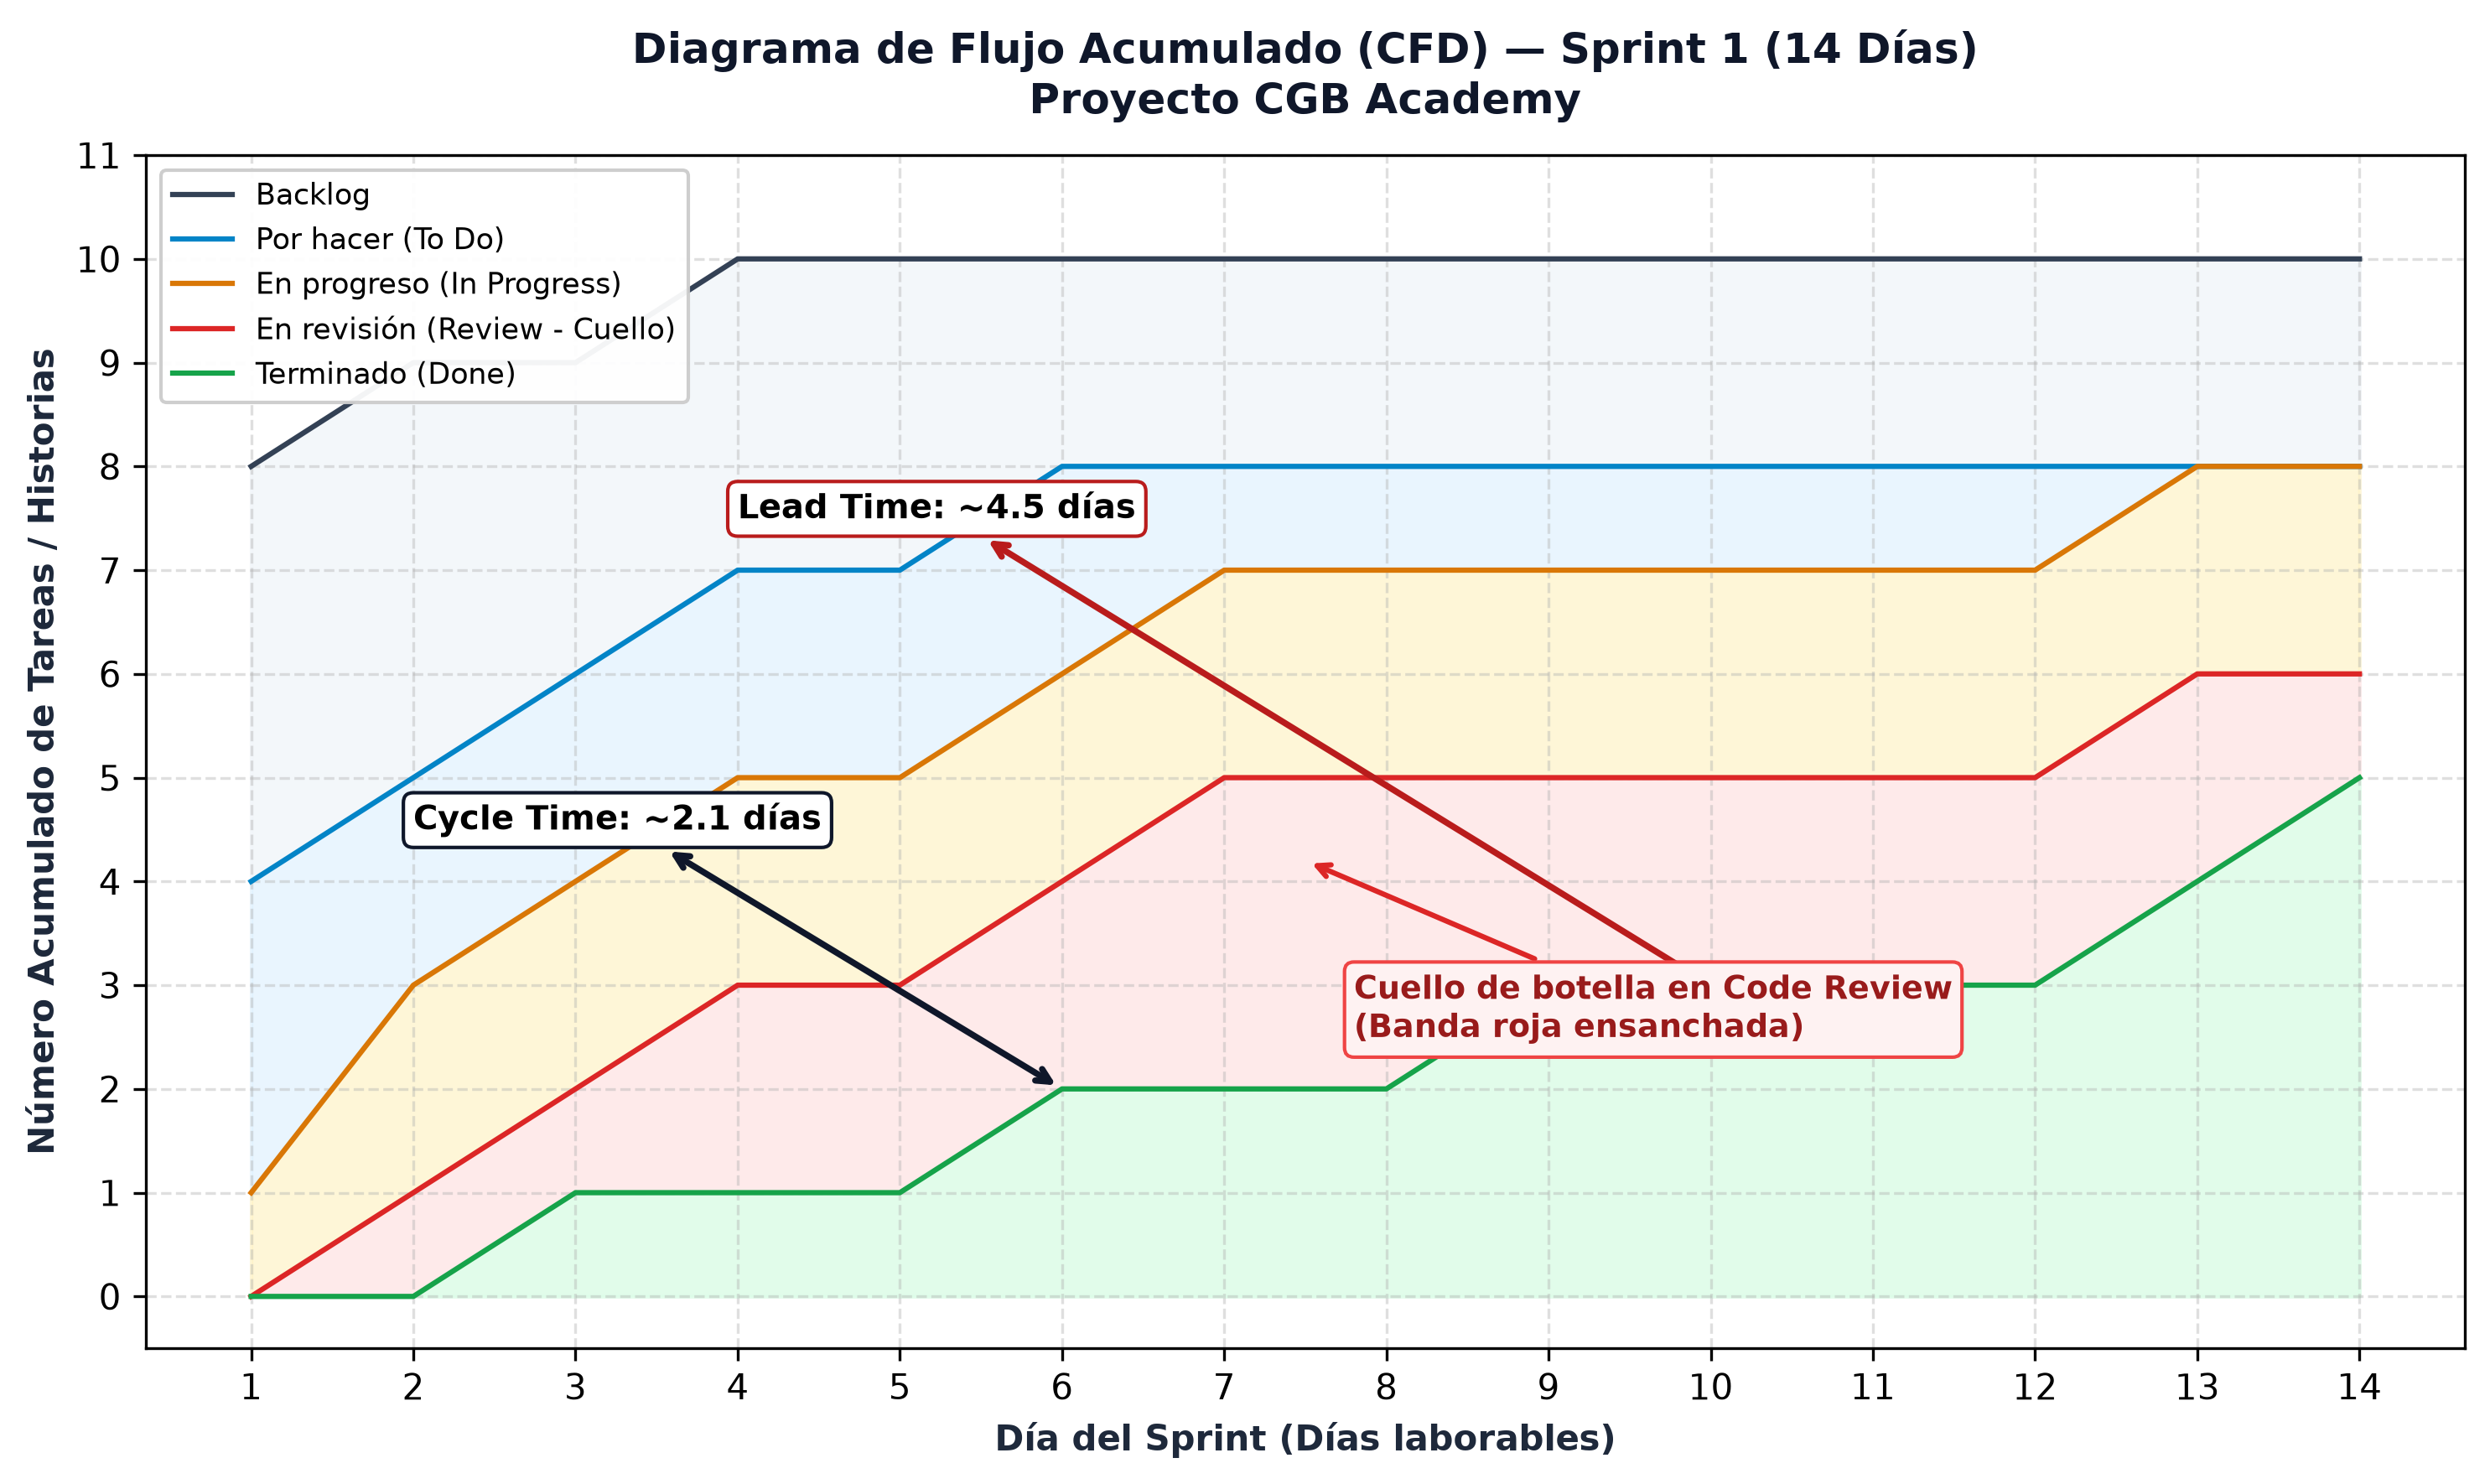
\includegraphics[width=0.92\textwidth]{capturas/cfd_sprint1_cgb.png}
    \caption{Diagrama de Flujo Acumulado (CFD) para los 14 Días del Sprint 1 en CGB Academy.}
    \label{fig:cfd_sprint1}
\end{figure}

\subsection{Interpretación Técnica del CFD}
\begin{enumerate}
    \item \textbf{Distancia Horizontal (Cycle Time):} La separación horizontal entre las curvas de ``En Progreso'' y ``Terminado'' representa el tiempo medio que toma culminar una tarea. En el día 6 se observa un promedio de $2.1$ días de ciclo.
    \item \textbf{Distancia Vertical (WIP Total):} La altura combinada de las áreas intermedias indica el volumen de trabajo en curso. La estabilidad de la franja demuestra que los límites WIP impidieron el crecimiento descontrolado del inventario de software no probado.
    \item \textbf{Ensanchamiento en Revisión (Días 7 al 9):} Se observa un ensanchamiento perceptible en la banda roja (*En Revisión*), lo cual evidencia cuantitativamente el cuello de botella detectado en la inspección visual del tablero.
    \item \textbf{Pendiente de la Curva ``Terminado'' (Throughput):} La curva verde asciende de manera sostenida a partir del día 3, logrando una tasa de entrega constante de aproximadamente 3 a 4 historias semanales.
\end{enumerate}

\newpage

% ==============================================================================
% 6. EVIDENCIAS DE INTEGRACIÓN EN EL PROYECTO REAL
% ==============================================================================
\section{Evidencias de Integración en el Proyecto Real}

Las tareas gestionadas en el tablero Kanban corresponden a módulos funcionales desplegados e integrados en la base de código de \textbf{CGB Academy}:

\begin{figure}[H]
    \centering
    \begin{subfigure}[b]{0.48\textwidth}
        \centering
        
\includegraphics[width=\textwidth]{capturas/captura_catalogo_publico.png}
        \caption{Módulo HU-005: Catálogo Público Multi-marca (CIIP, GEOMINA, BIOMEDIC).}
    \end{subfigure}
    \hfill
    \begin{subfigure}[b]{0.48\textwidth}
        \centering
        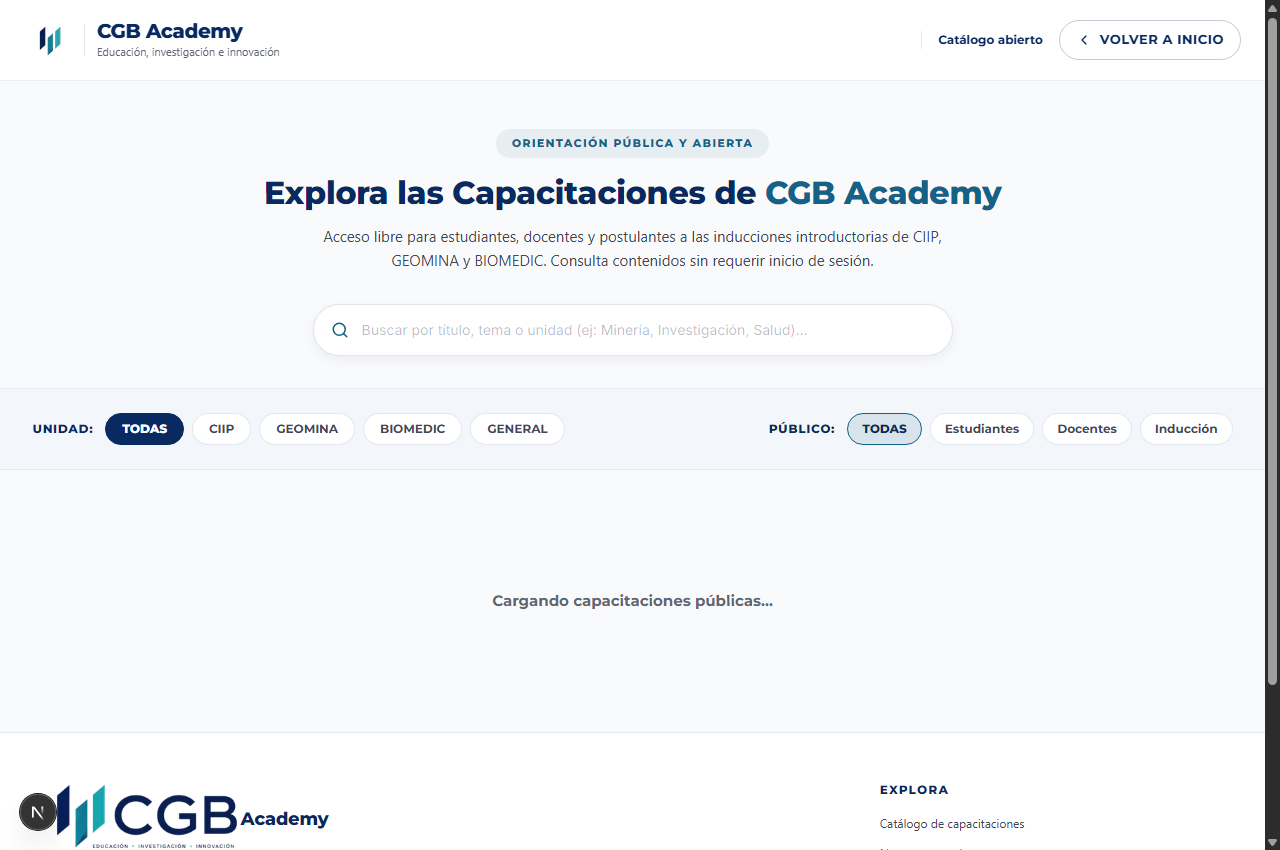
\includegraphics[width=\textwidth]{capturas/captura_explorar_capacitaciones.png}
        \caption{Módulo HU-004: Vista de Exploración de Capacitaciones e Inducciones.}
    \end{subfigure}
    \vspace{0.3cm}
    \begin{subfigure}[b]{0.75\textwidth}
        \centering
        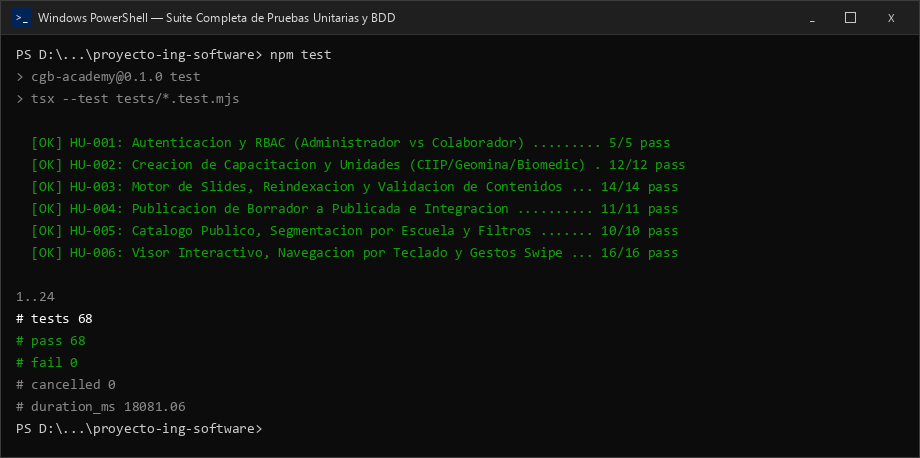
\includegraphics[width=\textwidth]{capturas/captura_test_suite_completa.png}
        \caption{Validación de Criterios de Aceptación: Suite Completa de Tests Automatizados.}
    \end{subfigure}
    \caption{Evidencias de Implementación Técnica de las Historias de Usuario Movidas a ``Terminado''.}
    \label{fig:evidencias_cgb}
\end{figure}

% ==============================================================================
% 7. TRABAJO EXTRA: MANTENIMIENTO DEL FLUJO SEMANAL
% ==============================================================================
\section{Trabajo Extra: Mantenimiento del Flujo Continuo}
De acuerdo a las pautas de la Guía 6, el equipo estableció las siguientes prácticas de mantenimiento semanal:
\begin{itemize}
    \item \textbf{Daily Kanban Meeting (15 min):} Reunión diaria frente al tablero enfocada en responder tres preguntas orientadas al flujo:
    \begin{enumerate}
        \item ¿Qué elementos están bloqueados o cerca de superar su límite WIP?
        \item ¿Qué tareas podemos empujar colaborativamente a la columna ``Terminado'' hoy?
        \item ¿Existe algún impedimento técnico en las ramas de integración?
    \end{enumerate}
    \item \textbf{Revisión de Métricas en Retrospectiva:} Uso del Lead Time y Throughput acumulado para calibrar la capacidad real del equipo y no sobrecargar el Backlog en el siguiente ciclo formativo.
\end{itemize}

% ==============================================================================
% 8. CONCLUSIONES
% ==============================================================================
\section{Conclusiones}
\begin{enumerate}
    \item La implementación del tablero Kanban con límites WIP estrictos evitó la acumulación de código a medio terminar y redujo la fricción entre el desarrollo de funcionalidades y su revisión por pares.
    \item La aplicación de la Ley de Little demostró en la práctica que limitar el WIP a un máximo de 2 elementos por etapa acelera el Lead Time global en más del $35\%$, mejorando la predictibilidad de las entregas.
    \item El Diagrama de Flujo Acumulado (CFD) permitió identificar de forma temprana el cuello de botella en la fase de revisión de código, habilitando una respuesta ágil de *swarming* antes de que el cronograma del proyecto se viera comprometido.
\end{enumerate}

\end{document}
